
    The Compiler Analysis Description Language (CAnDL) makes the constraint
    methodology from \Cref{chapter:theory} accessible to the Clang compiler
    within the LLVM compiler infrastructure.
    The previous chapter showed how this enables compiler analysis tools to be
    generated from declarative specifications, replicating and extending
    established compiler abilities.
    This chapter goes beyond restating and improving existing functionality.
    Instead, it implements automatic parallelisation methods for programs that
    were previously inaccessible to compiler reasoning.

    Complex Reduction and Histogram Computations (CReHCs) are identified as a
    previously overlooked  {\em computational idiom}.
    CReHCs constitute performance bottlenecks of important benchmark programs
    and share algorithmic structure that allows for targeted acceleration and
    parallelisation approaches.
    In contrast to the better-understood scalar reductions, CReHCs may contain
    indirect memory accesses and non-trivial control flow.
    Such loops have not typically been studied as a single class of
    calculations, but this chapter demonstrates that grouping them together
    allows for automatic detection and parallelisation using shared methods.

    After introducing CReHCs, this chapter presents the Idiom Description
    Language (IDL) as an extension of CAnDL and uses it to implement the
    detection of this idiom.
    The additional language features of IDL enable capturing well-behaved
    kernel functions.
    CReHCs contain reduction operators that are modelled as kernel functions,
    but kernel functions are also required in the formulation of other
    computational idioms, such as stencil codes.
    
    Grouping reductions and histograms together and formulating CReHCs in IDL
    enables their automatic recognition in C/C++ program code.
    The evaluation section shows results from benchmarking the outcomes of
    parallelisation routines that were implemented to complement the detection.
    Significant speedups were achieved on several programs from the
    NAS Parallel Benchmark suite, the Parboil Benchmarks, and Rodinia.

\section{Introduction}

    Reductions occur widely in numerical applications.
    Parallelisation techniques for them were established by
    \citet{rauchwerger1999lrpd,yu2006adaptive,Jradi2017fast}, and others.
    Typical reductions successively apply an arithmetic operator over an
    array of numeric values in order to compute, for example, the sum of a set
    of floating-point numbers.
    Perhaps most prominently, a reduction makes up the innermost loop of the
    matrix multiplication kernel in the form of a dot product.
    In this form, reductions are critical to high performance computing
    workloads based on linear algebra, as well as embedded benchmarks and
    emerging machine learning and computer vision applications
    \citep{Reddy2016Reduction}.
    Even so, linear algebra allows for much more targeted optimisation methods.
    Interpreting the innermost loop of matrix multiplication as an arbitrary
    reduction is unlikely to achieve comparable performance.

    However, there is a much larger class of computations that can be
    parallelised in much the same way.
    This is the class of Complex Reduction and Histogram Computations (CReHCs),
    a broad generalisation of conventional reductions that may also contain
    updates to dynamically selected elements in arrays.
    This manner of array access is characteristic for the calculation of
    histograms.
    CReHCs constitute an important set of standard program kernels.
    They typically have a higher arithmetic intensity and can be more profitably
    exploited on their own than simple scalar reductions.

    Discovering and exploiting scalar reductions in programs has been
    studied for many years, by \citet{pottenger1995idiom}, among others.
    The treatment of generalisations of reduction operations has received less
    attention.
    While some work has been published on parallelising such computations,
    automatic detection mostly evades established compiler analysis methods.
    The reason is that histogram reductions intrinsically contain indirect
    memory accesses, posing a challenge to compilers that use
    standard data dependence \citep{kuck1981dependence} or the polyhedral model
    \citep{benabderrahmane2010polyhedral} as the basis of their analysis.

    The constraint programming methodology derived in \Cref{chapter:theory},
    however, is not inhibited by such indirect memory accesses.
    \Cref{chapter:candl} developed the constraint programming language CAnDL
    using this methodology and showed that it could also recognise intricate
    control flow.
    This chapter presents the Idiom Detection Language (IDL) as an extension
    of CAnDL and uses it to implement the detection of CReHCs.
    The additional language features enable IDL to express well-behaved
    kernel functions, which capture the reduction operators of CReHCs.
    The IDL solver automatically identifies conforming subsets of LLVM IR during
    compilation.

    This chapter focuses on deriving the detection of reductions and assumes
    that later compiler stages are responsible for mapping this to dedicated
    code generation backends.
    Nevertheless, to illustrate the potential performance of the scheme, it also
    introduces a complementing code generation pass.
    This transformation pass achieved significant program-wide speedups on those
    benchmarks where reductions were performance bottlenecks.

\section{Motivation}

    \Cref{sum-figure} shows a standard scalar reduction.
    Inside a single loop, the elements of the array ``{\tt a}'' are
    successively accumulated in the variable ``{\tt sum}'' using the
    ``{\tt +=}'' operator.
    This accumulation creates dependencies between successive loop iterations.
    However, those are easy to break.
    Rather than sequentially accumulating ``{\tt a}'' into ``{\tt sum}'', it is
    possible to accumulate partial sums into thread-private copies of
    ``{\tt sum}'' in parallel, which are then added to form the final value.

\begin{figure}[h]
\begin{lstlisting}[language=MyCpp, label={sum-figure}, caption=
    {The most conventional example of a reduction is the adding up of values
     in an array:
     The reduction operator ``{\tt+}'' {\it reduces} the array ``{\tt a}'' to
     a single value -- the reduction variable ``{\tt sum}''.}]
sum = 0;
for(i = 0; i < n; i++)
  sum += a[i];
\end{lstlisting}
\end{figure}

    Simple scalar reductions frequently occur, and existing compilers readily
    exploit them.
    Despite their abundance, scalar reductions rarely dominate execution time,
    and when they do, they are often part of more prominent algorithms, such as
    matrix multiplication.
    This often makes outer-scope parallelism more profitable to exploit.
    Therefore, the parallelisation of simple reductions alone has only a
    limited impact on program performance.

    \Cref{complex-reduction-figure} shows a more complex section of code that
    constitutes a performance bottleneck of the ``Embarrassingly Parallel''
    benchmark program in the NAS Parallel Benchmarks.
    Note that the name of the benchmark refers to outer-loop parallelism.
    It is not directly evident that this computation can be treated as a
    reduction.
    However, it can be parallelised similarly to the simple sum.
    Creating thread-private copies of the reduction variables is again the
    critical step.

\begin{figure}[h]
\begin{lstlisting}[language=MyCpp, label={complex-reduction-figure}, caption=
   {Example of a Complex Reduction and Histogram Computation:
    The bottleneck from the NAS Parallel Benchmarks can be parallelised as a
    reduction by privatising ``{\tt sx}'', ``{\tt sy}'', ``{\tt q[]}''.}]
for(i = 0; i < NK; i++) {
  x1 = 2.0 * x[2*i] - 1.0;
  x2 = 2.0 * x[2*i+1] - 1.0;
  t1 = x1 * x1 + x2 * x2;
  if(t1 <= 1.0) {
    t2   = sqrt(-2.0 * log(t1) / t1);
    t3   = (x1 * t2);
    t4   = (x2 * t2);
    l    = MAX(fabs(t3), fabs(t4));
    q[l] = q[l] + 1.0;
    sx   = sx + t3;
    sy   = sy + t4;
  }
}
\end{lstlisting}
\end{figure}

    The loop in \Cref{complex-reduction-figure} is considered a CReHC for the
    following reasons:
    Firstly, there is an input array ``{\tt x[]}'', from which values are read
    successively in each iteration.
    Secondly, the values ``{\tt sx}'' and ``{\tt sy}'' are scalar reduction
    variables, as is evident from lines 11--12.
    They are incremented conditionally, and the added value is not merely
    ``{\tt x[i]}'' but the result of a complex calculation with control flow.
    Nonetheless, the calculation and the branching condition only depend on the
    input values ``{\tt x[2*i]}'' and ``{\tt x[2*i+1]}''.
    Thirdly, the array ``{\tt q[]}'' is updated as a histogram array at line 10.
    The index ``{\tt l}'' is not directly read from an input array, as in a
    conventional histogram, but again the calculation only depends on the input
    values.

    As in the case of the simple sum, the parallelisation of this code
    requires the computation of partial results in separate memory locations
    before merging the partial results.
    The whole process is illustrated in Figure \ref{nice-picture}, with
    different colours on the right showing the distribution of the program
    over two threads.
    The scalar variables ``{\tt sx}'', ``{\tt sy}'' and the array ``{\tt q[]}''
    are privatised.
    Partial results are then accumulated in the local copies by partitioning the
    input array equally across the two threads. 
    Finally, the threads are synchronised, and partial results merged.
    This is done by adding the local copies of ``{\tt sx}'', ``{\tt sy}'' and
    performing an element-wise addition of the local copies of ``{\tt q[]}''. 

\begin{figure}[t]
\centering
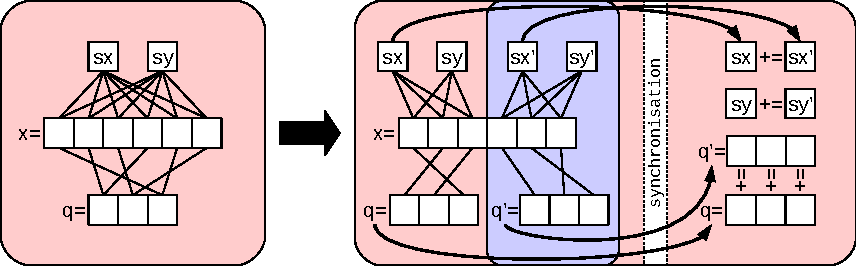
\includegraphics[width=\textwidth]{figures/parallelisereduction.pdf}
\caption{Parallelisation of \Cref{complex-reduction-figure}:
         The input ``{\tt x[]}'' is split over two threads (red/blue) that
         operate on private copies of ``{\tt sx}'', ``{\tt sy}'', ``{\tt q[]}''.
         These are merged after a synchronisation barrier.}
\label{nice-picture}
\end{figure}

\begin{figure}[p]
\centering
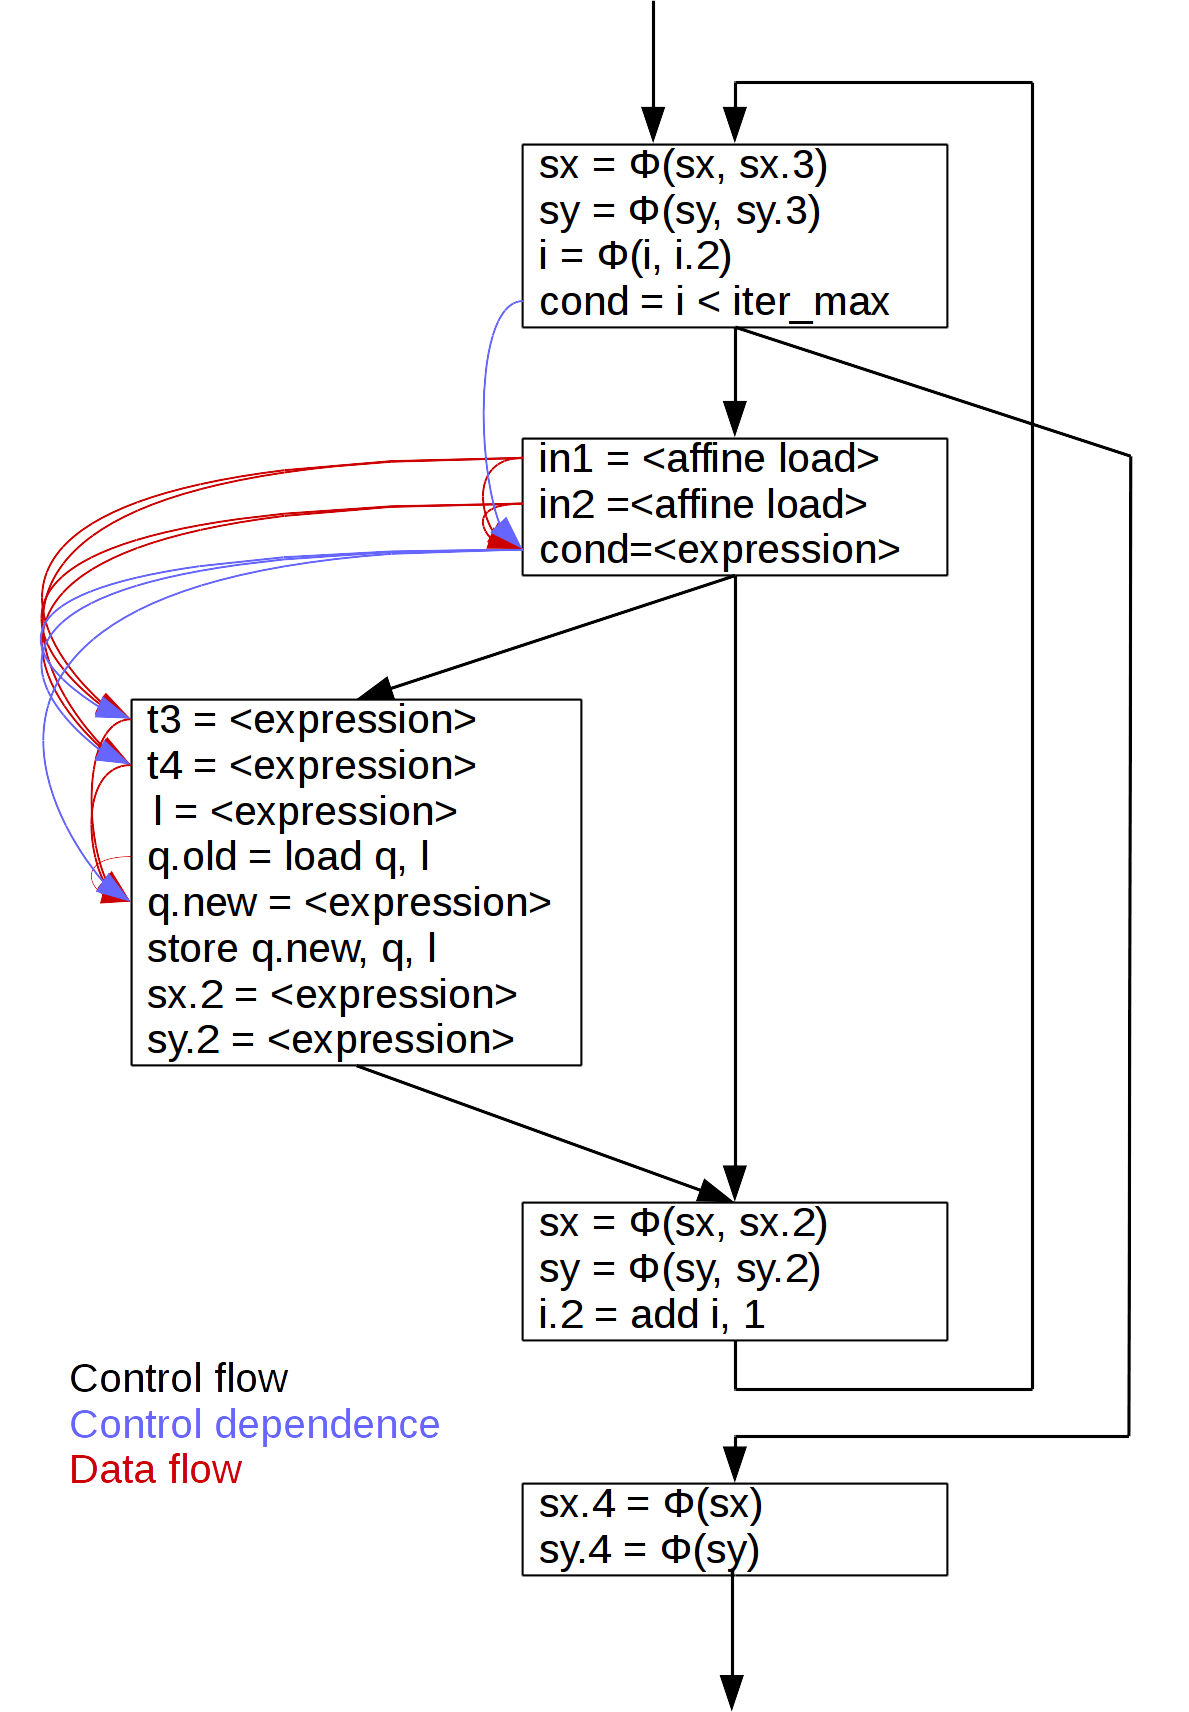
\includegraphics[width=\textwidth]{figures/nicepicture2.png}
\caption{Fragments of the data flow, control flow, and control dependencies in
         the internal compiler representation of the source code in
         \Cref{complex-reduction-figure}:
         These interactions must be considered when searching for code that
         implements Complex Reduction and Histogram Computations.}
\label{nice-picture2}
\end{figure}

    \Cref{nice-picture2} gives an insight into why existing schemes do not
    detect such reductions by showing the compiler representation of this 
    program.
    The histogram update occurs in the third basic block with the ``load'',
    assignment and ``store'' operations, but it is by no means obvious that this
    is a safe reduction.
    In fact, accurately detecting reductions is non-trivial.
    If in the original program, shown in \Cref{complex-reduction-figure}, the
    condition on line 5 was changed to ``{\tt t1 <= sx}'', this would be no
    longer be a sound reduction, as there would now be a control dependence on
    an intermediate result.
    This, in turn, would manifest itself as an additional data dependence edge
    from block 3 to block 2 in \Cref{nice-picture2}.
    Moreover, the code segment can only be classified as a reduction because
    all the function calls that are present are pure.
    Such details have to be checked to ensure correctness.
    What is needed is a way to specify these conditions precisely and to then
    automatically identify code regions that satisfy the constraints.

\section{Recognising CReHCs}

    There are three fundamental issues to address in exploiting CReHCs:
    detection, replacement, and profitability.
    This chapter focuses on the reliable detection of reductions.
    For evaluation purposes, a preliminary code generation phase that generates
    parallel code was implemented targeting the POSIX Threads interfaces.
    Smart profitability heuristics are essential in practice to determine
    whether or not to apply parallelising code transformations.
    For this work, a simple profile-based approach was used.

    In the following sub-sections, the properties that loops need to satisfy
    to be interpreted as CReHCs are derived.
    Conditions for sound CReHCs are established and demonstrated on
    counterexamples.
    These observations then motivate extensions to CAnDL that culminate in the
    Idiom Detection Language (IDL).
    This language eventually enables the constraint-based specification of
    CReHCs for automatic compiler detection.

\subsection{Constraint-Based Formulation}

    The motivation section described how CReHCs could be parallelised as
    reduction operations.
    For compilers to apply this parallelisation automatically, a precise
    specification of the suitable program loops is required.
    This section gives an overview of the necessary conditions for CReHCs, which
    are then precisely formulated in \Cref{sec:IDLdefinition,sec:IDLCReHCs}.

\subsubsection{Scalar Reductions}
\label{section:scalarcond}

    Informally, the following conditions are required to hold in a piece of
    source code for it to contain a computation that can be parallelised like a
    scalar reduction:
    \begin{enumerate}
        \item The code is contained in a for-loop, and the iteration space of
              the loop is known ahead of time
              (but not necessarily at compile time).
        \item There is a scalar value $x$ that is updated in every iteration.
        \item One or multiple values $a_1,\dots,a_n$ are read from arrays, and
              the access indices are affine in the loop iterator.
        \item The updated value $x'$ is computed as a term only of $x$, the
              array values $a_1,\dots,a_n$, and of values that are constant
              within the loop.
    \end{enumerate}

    This definition is broader than usual.
    In particular, it allows the reduction to encompass multiple input arrays.
    Furthermore, complex computations inside the reduction are possible, not
    just binary scalar operators.
    Note that condition 2 is enforced only at SSA level.
    Finally, this definition does not yet contain a commutativity condition that
    would be necessary to allow the parallelisation to work.
    Instead, it also captures intrinsically sequential scalar reductions.

    \paragraph*{Example}
    Both ``{\tt sx}'' and ``{\tt sy}'' in \Cref{complex-reduction-figure}
    satisfy the conditions.
    Firstly, the iteration space of the loop is bounded by ``{\tt NK}'', which
    is constant.
    Secondly, within the SSA representation, both ``{\tt sx}'' and ``{\tt sy}''
    are unconditionally updated via $\Phi$-instructions, shown
    in \Cref{nice-picture2}.
    This is despite the conditional statement in the original C representation
    of the program.
    Thirdly, two values are read from the single input array ``{\tt x[]}'' in
    every iteration, and the indices ``{\tt 2*i}'' and ``{\tt 2*i+1}'' are
    affine in ``{\tt i}''.
    Finally, the updated values depend only on their respective old values,
    the two values read from ``{\tt x[]}'', and the constants
    ``{\tt 1.0}'' and ``{\tt 2.0}''.
    This also relies on the fact that all functions used in the computation are
    pure functions.

\begin{figure}[t]
\begin{lstlisting}[language=MyCpp]
sum = 0;
for(i = 0; i < n && sum < 10; i++)
    sum += a[i];
\end{lstlisting}
\begin{lstlisting}[language=MyCpp]
sum = 0;
for(i = 0; i < n; i++)
    b[i] += a[i];
\end{lstlisting}
\begin{lstlisting}[language=MyCpp]
chase = 0;
for(i = 0; i < n; i++)
    chase = a[chase];
\end{lstlisting}
\begin{lstlisting}[language=MyCpp,label={counterexamples},caption=
   {Counterexamples to the four conditions: None of these computations can be
    parallelised as scalar reductions.
    The first and last example implement the same program.}]
sum = 0;
active = true;
for(i = 0; i < n; i++) {
    sum += active?a[i]:0;
    active = active && (sum < 10);
}
\end{lstlisting}
\end{figure}

    \paragraph*{Counterexamples}
    \Cref{counterexamples} shows counterexamples to the four conditions,
    demonstrating why they are all needed in order to parallelise a given
    computation as a scalar reduction.

    In the first example, the iteration space is not known in advance, as the
    computation can be terminated depending on the input data.
    This makes it impossible to compute partial sums in parallel.
    The second example is straightforward, as there is no reduction variable
    that could be privatised.
    The loop could still be computed in parallel -- but not as a scalar
    reduction.
    The third example uses index calculations that are not affine in
    ``{\tt i}''.
    This prevents a straightforward distribution of the input array across
    threads.
    In this particular case, the index calculation also involves values other
    than ``{\tt i}'', preventing the computation of partial results entirely.
    The final example is equivalent to the first but breaks the fourth condition
    instead of the first.

\subsubsection{Histogram Reductions}
\label{section:histocond}

    The conditions that apply to histogram reductions are similar to those for
    scalar reductions.
    However, instead of one function parameter, there are two:
    \begin{enumerate}
        \item The code is contained in a for-loop, and the iteration space of
              the loop is known ahead of time
              (but not necessarily at compile time).
        \item One or multiple values $a_1,\dots,a_n$ are read from arrays, and
              the access indices are affine in the loop iterator.
        \item An integer $k$ is computed as a term only of the array values
              $a_1,\dots,a_n$, and of values that are constant within the loop.
        \item A value $x$ is read from an array at index $k$ and a
              modified value $x'$ is written at the same index.
              The writing may be control-dependent only on $a_1,\dots,a_n$ and
              it may not be in a nested loop.
        \item The updated value $x'$ is computed as a term only of $x$, the
              array values $a_1,\dots,a_n$, and of values that are constant
              within the loop.
    \end{enumerate}

    Histogram reductions are only parallelisable if their update operator is
    commutative, just as is the case for scalar reductions.
    However, checking this condition requires a post-processing step,
    which is independent of the detection of the algorithmic structure.
    For this research, checking commutativity was considered the responsibility
    of code generation.

    \paragraph*{Example}
    The first two conditions are the same as those in the previous discussion of
    scalar reductions and were shown to hold for the loop in
    \Cref{complex-reduction-figure}.
    The array ``{\tt q[]}'' also satisfies the remaining conditions.
    Firstly, the variable ``{\tt l}'' corresponds to the index $k$.
    Secondly, the element ``{\tt q[l]}'' is read, modified and written.
    Lastly, the updated value is computed in an allowed fashion, as it is
    obtained by merely adding a constant ``{\tt 1.0}'' to the previous value.

    \paragraph*{Counterexamples}
    Again, counterexamples are given in \Cref{counterexamples2} to develop an
    intuition about the significance of conditions 3--5.

    In the first example, the index of the histogram is not computed from an
    input array but instead read from an input stream.
    This makes parallelisation as a histogram impossible, as the stream is only
    available sequentially.
    In the second and third examples, the computation effectively stops when an
    index beyond a threshold size occurs.
    This can only be accounted for by sequentially going through the array.
    Therefore, the parallel computation of partial results is not efficiently
    possible.
    This behaviour is evoked in two different ways, by breaking the conditions
    4 and 5, respectively.
    This shows the need to restrict both the data flow and control flow of the
    histogram kernel.

\begin{figure}[t]
\lstset{
 basicstyle = \linespread{0.883}\ttfamily
}
\begin{lstlisting}[language=MyCpp]
for(i = 0; i < n; i++)
    hist[getchar()] += 1;
\end{lstlisting}
\begin{lstlisting}[language=MyCpp]
active = true;
for(i = 0; i < n; i++) {
    if(a[i] > 9)
        active = false;
    if(active)
        hist[a[i]] += 1;
}
\end{lstlisting}
\begin{lstlisting}[language=MyCpp,label={counterexamples2},caption=
   {Counterexamples to the last three conditions:
    None of these computations can be parallelised as histograms.
    The final two example loops implement equivalent functionality.}]
active = true;
for(i = 0; i < n; i++) {
    if(a[i] > 9)
        active = false;
    hist[a[i]] += active?1:0;
}
\end{lstlisting}
\end{figure}

\subsection{The Idiom Detection Language}
\label{sec:IDLdefinition}

    For automatic detection during compilation, the conditions from
    \Cref{section:histocond,section:scalarcond} are specified formally in
    a constraint language.
    CAnDL from \Cref{chapter:candl} is taken as the basis for this formulation.
    However, additional language constructs are required in order to capture
    the kernel computations.

    This extension of CAnDL leads to the definition of the
    Idiom Detection Language (IDL).
    IDL uses the solver infrastructure of CAnDL and retains the same high-level
    program structure.
    However, it extends the language and modifies the syntax to be more
    convenient for large-scale specifications, replacing uncommon Unicode
    characters.
    \Cref{CanDLtoIDL} shows syntax differences.\footnote{The complete grammar
    file that was used to generate the parser of the IDL compiler is in
    Appendix~\ref{appendix:IDLgrammar}.}

\begin{table}[H]
    \lstset{keepspaces}
    \centering
    \definecolor{tableShade}{gray}{0.8}
    \rowcolors{1}{}{tableShade}
    \begin{tabular}{p{0.39\textwidth}p{0.553\textwidth}}
        \toprule
        {\bf CAnDL} & {\bf IDL}\\
        \midrule
        {\lstinline[language=CAnDL]!∧!}, {\lstinline[language=CAnDL]!∨!} &
        {\lstinline[language=IDL]!and!}, {\lstinline[language=IDL]!or!} \\
        {\lstinline[language=CAnDL]!include Spec({A}->{B}!}, \vspace{-2.5mm}\newline
        {\phantom{\lstinline[language=CAnDL]!include Spec(!}\lstinline[language=CAnDL]!{C}->{D})@{E}!} &
        {\lstinline[language=IDL]!inherits Spec with {A} as {B}!} \vspace{-2.5mm}\newline
        {\phantom{\lstinline[language=IDL]!inherits Spec!}\hspace{4.4mm}\lstinline[language=IDL]!and {C} as {D} at {E}!}\\
        {\lstinline[language=CAnDL]!{A}={B}!},
        {\lstinline[language=CAnDL]!{A}≠{B}!} &
        {\lstinline[language=IDL]!{A} is [ !\ttfamily{not}\lstinline[language=IDL]! ] equal to {B}!} \\
        {\lstinline[language=CAnDL]!domination({A},{B})!} &
        {\lstinline[language=IDL]!{A} control flow dominates {B}!} \\
        {\lstinline[language=CAnDL]!opcode{A} = store!} &
        {\lstinline[language=IDL]!{A} is store instruction!} \\
        {\lstinline[language=CAnDL]!{A} ∈ {B}.args!} &
        {\lstinline[language=IDL]!{A} has data flow to {B}!} \\
        \bottomrule
    \end{tabular}
    \caption{The Idiom Detection Language (IDL) is derived from CAnDL.
             However, it uses a more descriptive syntax, without uncommon
             Unicode characters such as ``$\land$'', ``$\lor$'', ``$\in$'',
             and ``$\neq$''.}
    \label{CanDLtoIDL}
\end{table}

\subsubsection{Kernel Functions as Generalised Domination}

    Complex Reduction and Histogram Computations can be expressed as a
    higher-order function.
    This means that the computational idiom is not just parameterised with
    numerical values, such as array dimensions, but contains kernel functions
    as parameters.
    To enable the capture of such higher-order functions in IDL, additional
    constraint expressions are required that go beyond what CAnDL
    provided.

    Specifically, IDL adds another atomic constraint based on generalised graph
    domination, as previously described in \Cref{def:domconstr}, using the
    following syntax:
\begin{figure}[h]
    \centering
    \begin{tabular}{|c|}
        \hline
        $\textbf{all flow from }\text{\it variable\_tuple}\textbf{ or any origin to any of }\text{\it variable\_tuple}$\\
        $\textbf{ passes through at least one of }\text{\it variable\_tuple}$\\
        \hline
    \end{tabular}
\end{figure}

    \noindent
    The syntax of this atomic constraint is quite descriptive, but some
    details require explanation.
    Firstly, ``flow'' in this constraint does not only capture data flow.
    To cover kernel functions with non-trivial control flow, the
    underlying graph on which this constraint operates is formed as an extension
    of the data flow graph $DFG_\mathcal F^*$.
    In addition to the data flow edges, it has an edge from each branch
    instruction to every instruction within all its targeted basic blocks.
    Secondly, as opposed to the control flow graph that is typically considered
    for dominance relationships, the resulting graph has no distinguished single
    ``origin''.
    Aside from the control entry, all non-pure function calls and reads from
    memory are considered graph origins.

    \Cref{kernelexample} demonstrates the significance of this definition.
    At the top is an SSA pseudocode representation of the complex reduction and
    histogram calculation from \Cref{complex-reduction-figure}, annotated in the
    right column with all the dependencies described above.
    It is now possible to check the validity of the kernel function that is used
    within the loop for the reduction on ``{\tt sx}'' as follows:
    
\begin{figure}[h]
    \centering
    \begin{lstlisting}[language=IDL]
([all]) flow from {loop_carried[0..3]} ([or]) any origin
    to any of {sx''} passes through ([at]) least one of
    {sx,t2,t5,precursor,backedge,outside[0..N]}}
    \end{lstlisting}
\end{figure}

    \noindent
    This use of the new atomic constraint requires several additional
    conditions:
    ``{\tt precursor}'' and ``{\tt backedge}'' should be determined and
    ``{\tt outside[0..N]}'' should contain all origins that lie outside
    the SESE region within which the kernel functions is considered.
    Furthermore, the array ``{\tt loop\_carried}'' needs to be constrained to
    contain all loop-carried $\Phi$-instructions.

    With this setup, it is straightforward to check that the constraint is
    satisfied.
    Control flow can only reach $sx''$ via the precursor at line 1 and the
    back edge at line 28.
    The other relevant graph origins for this example are the load
    instructions at lines 6,9,18 and the explicitly added $\Phi$-instructions.
    The three of these that can reach $sx''$ through the graph are explicitly
    killed as generalised dominators ``{\tt sx}'', ``{\tt t2}'', and
    ``{\tt t5}''.

\begin{figure}[p]
\centering
\begin{tabular}{|c|rl|l|}
\hline
\multicolumn{1}{|c}{\bf Block} &  \multicolumn{2}{|c|}{\bf Operation} & \multicolumn{1}{c|}{\bf Dependencies} \\
\hline
\hline
\multirow{1}{*}{\bf entry}
  & {\bf 1:} & \textcolor{color_strings}{$\text{goto }loop$}&\textcolor{color_strings}{\bf outside the considered region}\\
\hline
\multirow{9}{*}{\bf loop\vspace{4.5mm}}
  & {\bf  2:} & \textcolor{gray}{$i\leftarrow \Phi(entry:0,\ loop:i')$}&\textcolor{gray}{loop carried data flow}\\[-1.7mm]
  & {\bf  3:} & \textcolor{color_types}{$sx\leftarrow \Phi(entry:0.0,\ loop:sx'')$}&\textcolor{color_types}{\bf loop carried data flow}\\[-1.7mm]
  & {\bf  4:} & \textcolor{gray}{$sy\leftarrow \Phi(entry:0.0,\ loop:sy'')$}&\textcolor{gray}{loop carried data flow}\\[-1.7mm]
  & {\bf  5:} & \textcolor{gray}{$t_1\leftarrow 2\cdot i$}&\textcolor{gray}{control({\bf 1, 28}), data({\bf 2})}\\[-1.7mm]
  & {\bf  6:} & \textcolor{color_types}{$t_2\leftarrow\textbf{load }x[t_1]$}&\textcolor{color_types}{\bf origin of data flow}\\[-1.7mm]
  & {\bf  7:} & $t_3\leftarrow 2.0\cdot t_2-1.0$&{\bf control({\bf 1, 28}), data({\bf 6})}\\[-1.7mm]
  & {\bf  8:} & \textcolor{gray}{$t_4\leftarrow 2\cdot i+1$}&\textcolor{gray}{control({\bf 1, 28}), data({\bf 2})}\\[-1.7mm]
  & {\bf  9:} & \textcolor{color_types}{$t_5\leftarrow\textbf{load }x[t_4]$}&\textcolor{color_types}{\bf origin of data flow}\\[-1.7mm]
  & {\bf 10:} & $t_6\leftarrow 2.0\cdot t_5-1.0$&{\bf control({\bf 1, 28}), data({\bf 9})}\\[-1.7mm]
  & {\bf 11:} & $t_7\leftarrow t_3\cdot t_3+t_6\cdot t_6$&{\bf control({\bf 1, 28}), data({\bf 7, 10})}\\[-1.7mm]
  & {\bf 12:} & $t_8\leftarrow t_7\leq1.0$&{\bf control({\bf 1, 28}), data({\bf 11})}\\[-1.7mm]
  & {\bf 13:} & $\text{if }t_8\text{ goto }ifblock\text{ else }uncond$&{\bf control({\bf 1, 28}), data({\bf 12})}\\
\hline
\multirow{8}{*}{\bf ifblock\vspace{3mm}}
 & {\bf 14:} & $t_9\leftarrow sqrt(-2.0\cdot log(t_7) / t_7)$&{\bf control({\bf 13}), data({\bf 11})}\\[-1.7mm]
 & {\bf 15:} & $t_{10}\leftarrow t_3*t_9$&{\bf control({\bf 13}), data({\bf 7, 14})}\\[-1.7mm]
 & {\bf 16:} & \textcolor{gray}{$t_{11}\leftarrow t_6\cdot t_9$}&\textcolor{gray}{control({\bf 13}), data({\bf 10, 14})}\\[-1.7mm]
 & {\bf 17:} & \textcolor{gray}{$l\leftarrow MAX(fabs(t_{10}), fabs(t_{11}))$}&\textcolor{gray}{control({\bf 13}), data({\bf 15, 16})}\\[-1.7mm]
 & {\bf 18:} & \textcolor{gray}{$t_{12}\leftarrow\textbf{load }q[l]$}&\textcolor{gray}{origin of data flow}\\[-1.7mm]
 & {\bf 19:} & \textcolor{gray}{$t_{13}\leftarrow t_{12}+1$}&\textcolor{gray}{control({\bf 13}), data({\bf 18})}\\[-1.7mm]
 & {\bf 20:} & \textcolor{gray}{$\textbf{store }q[l]\leftarrow t_{13}$}&\textcolor{gray}{control({\bf 13}), data({\bf 19})}\\[-1.7mm]
 & {\bf 21:} & $sx'\leftarrow sx+t_{10}$&{\bf control({\bf 13}), data({\bf 3, 15})}\\[-1.7mm]
 & {\bf 22:} & \textcolor{gray}{$sy'\leftarrow sy+t_{11}$}&\textcolor{gray}{control({\bf 13}), data({\bf 4, 16})}\\[-1.7mm]
 & {\bf 23:} & $\text{goto }uncond$&{\bf control({\bf 13})}\\
\hline
\multirow{4}{*}{\bf uncond\vspace{0.5mm}}
 & {\bf 24:} & \textcolor{color_keywords}{$sx''\leftarrow\Phi(loop:sx,\ ifblock:sx')$}&\textcolor{color_keywords}{\bf control({\bf 13, 23}), data({\bf 3, 21})}\\[-1.7mm]
 & {\bf 25:} & \textcolor{gray}{$sy''\leftarrow\Phi(loop:sy,\ ifblock:sy')$}&\textcolor{gray}{control({\bf 13, 23}), data({\bf 4, 22})}\\[-1.7mm]
 & {\bf 26:} & \textcolor{gray}{$i'\leftarrow i+1$}&\textcolor{gray}{control({\bf 13, 23}), data({\bf 2})}\\[-1.7mm]
 & {\bf 27:} & \textcolor{gray}{$t_{14}\leftarrow i' < NK$}&\textcolor{gray}{control({\bf 13, 23}), data({\bf 26})}\\[-1.7mm]
 & {\bf 28:} & \textcolor{color_strings}{$\text{if }t_{14}\text{ goto }loop\text{ else }exit$}&\textcolor{color_strings}{\bf outside the considered region}\\
\hline
\end{tabular}

\begin{tabular}{|cl|}
\multicolumn{2}{c}{{\bf function} kernel($sx, t_2, t_5$)}\\
\hline
\multirow{4}{*}{\bf entry\vspace{0.5mm}}
 & $t_3 \leftarrow 2.0\cdot t_2-1.0$\\[-1.7mm]
 & $t_6 \leftarrow 2.0\cdot t_5-1.0$\\[-1.7mm]
 & $t_7 \leftarrow t_3\cdot t_3+t_6\cdot t_6$\\[-1.7mm]
 & $t_8 \leftarrow t_7\leq 1.0$\\[-1.7mm]
 & $\text{if }t_8\text{ goto }ifblock\text{ else }uncond$\\
\hline
\multirow{4}{*}{\bf ifblock\vspace{4mm}}
 & $t_9\leftarrow sqrt(-2.0\cdot log(t_7) / t_7)$\\[-1.7mm]
 & $t_{10}\leftarrow t_3\cdot t_9$\\[-1.7mm]
 & $sx'\leftarrow sx+t_{10}$\\[-1.7mm]
 & $\text{goto }uncond$\\
\hline
\multirow{2}{*}{\bf uncond\vspace{2mm}}
 & $sx''\leftarrow\Phi(entry:sx,\ ifblock:sx')$\\[-1.7mm]
 & $\text{return }sx''$\\
\hline
\end{tabular}
\caption{A kernel function is identified within the SSA pseudocode at the top
    (cf.\ \Cref{complex-reduction-figure}):
    The value of $sx''$ is calculated in the SESE region spanning lines 2--27
    as a pure function of only \mbox{$sx$, $t_2$, and $t_5$}.
    This is determined by starting from $sx''$
    (\textcolor{color_keywords}{\bf blue}) and following the dependencies on the
    right, checking that all paths end in the predetermined function arguments
    \mbox{$sx$, $t_1$ and $t_5$ (\textcolor{color_types}{\bf red})}.
    The kernel function can then be extracted and valid SSA
    reconstructed, as shown at the bottom.}
\label{kernelexample}
\end{figure}

\begin{figure}[p]
\lstset{
 basicstyle = \linespread{1.173}\ttfamily
}
\begin{lstlisting}[language=IDL]
Constraint KernelFunction
( collect i  4 ( {entries[i]} has control
                     flow to {scope.begin}) and
  collect i 24 ( inherits LocalConst
                     with {scope} as {scope}
                                  at {outside[i]} and
                 {outside[i].value}
                     is ([not]) a numeric constant and
                 {outside[i].value} has data
                     flow to {outside[i].use} and
                 {scope.begin} control flow
                     dominates {outside[i].use}) and
  collect i  8 ( {loop_carried[i].update} reaches
                     phi node {loop_carried[i].value}
                     from {scope.end} and
                 {scope.begin} control flow
                     dominates {loop_carried[i].value}) and
  ([all]) flow from {loop_carried[0..8].value} ([or]) any origin
      to any of {result} passes through ([at]) least one of
      {inputs[0..32],entries[0..4],outside[0..24].value})
End
\end{lstlisting}
\begin{lstlisting}[language=IDL,label={IDLscalarPart},caption=
   {IDL specifications of a kernel function and a scalar reduction within a
    CReHC:
    In ``{\tt ScalarPart}'', the kernel function operates in a loop.
    Its input ``{\tt kernel.inputs}'' is composed of ``{\tt read\_values}'' and
    the reduction value of the previous iteration, concatenated with
    ``{\tt Concat}''.}]
Constraint ScalarPart
( {kernel.result} reaches phi node
      {old_value} from {loop.end} and
  inherits ScopeValue
      with {loop}      as {scope}
       and {old_value} as {value} and
  {kernel.result} has data flow to {final_value} and
  {loop.end} strictly control flow
      dominates {final_value} and
  inherits KernelFunction
      with {loop} as {scope} at {kernel} and
  inherits Concat(N1=31,N2=1)
      with {read_values}   as {in1}
       and {old_value}     as {in2}
       and {kernel.inputs} as {out})
End
\end{lstlisting}
\end{figure}

\subsubsection{Expressing Kernel Functions in IDL}

    \Cref{IDLscalarPart} encapsulates kernel functions as an IDL constraint
    specification in the top half.
    The specification is built around the previously introduced generalised
    graph domination constraint, which is invoked at lines 18--20.
    The arrays that are used in these final lines of the specification are
    filled with several collect-all statements at lines 2--17.
    Lines 2--3 collect all the entry points of the control flow.
    In the previous example, these were ``{\tt precursor}'' and
    ``{\tt backedge}''.
    All values from outside the scope that are used within the scope are
    collected at lines 4--12.
    These values can be considered the closure of the kernel function.
    Finally, lines 13--17 collect all the loop-carried $\Phi$-instructions,
    which only exist in case the scope is a loop.

    The bottom of \Cref{IDLscalarPart} shows the IDL specification of a
    scalar reduction component within a CReHC loop.
    This IDL specification is built around a kernel function, incorporating the
    specification at lines 10--11.
    The arguments to this kernel are set using the ``{\tt Concat}''
    specification at lines 12--15.
    This kernel function is connected with a loop-carried $\Phi$-instruction
    at lines 2--6.
    Finally, lines 7--9 make sure that the reduction value eventually leaves the
    loop, excluding loop-carried iterators that are only used within the loop.

    \autoref{IDLhistoPart} shows how histogram reductions are specified
    similarly.
    Two kernel functions calculate the index of the bin in the histogram
    (lines 7--9) and the updated value of its contents (lines 10--15).
    The histogram update in each iteration may be conditional, as expressed with
    ``{\tt ConditionalReadModifyWrite}'' in lines 2--6.
    Crucially, the kernel functions use the scope of the loop and already
    restrict this conditional to only depend on the allowed values.

\begin{figure}[H]
\lstset{
 basicstyle = \linespread{1.062}\ttfamily
}
\begin{lstlisting}[language=IDL,label={IDLhistoPart},caption=
   {IDL specification of a histogram reduction in a Complex Reduction and
    Histogram Computation:
    Two kernel functions are present.
    Lines 7--9 calculate the index into the histogram array, lines 10--11
    generate the updated value.
    The read-modify-write step may be conditional.}]
Constraint HistoPart
( inherits ConditionalReadModifyWrite
      with {loop}              as {scope}
       and {idx_kernel.result} as {address}
       and {val_kernel.result} as {new_value}
                               at {update} and
  inherits KernelFunction
      with {loop}        as {scope}
       and {read_values} as {inputs} at {idx_kernel} and
  inherits KernelFunction
      with {loop} as {scope} at {val_kernel} and
  inherits Concat(N1=31,N2=1)
      with {read_values}       as {in1}
       and {update.old_value}  as {in2}
       and {val_kernel.inputs} as {out})
End
\end{lstlisting}
\end{figure}

\subsection{Specification of CReHCs in IDL}
\label{sec:IDLCReHCs}

    \Cref{IDLcomplexred} shows how the previously described IDL specifications
    can be assembled to define the class of Complex Reduction and Histogram
    Computations.\footnote{The complete IDL code for this section is in
    Appendix~\ref{appendix:IDLreductions}.}

    Such computations are always encapsulated by a single for-loop, as
    stipulated at line 2.
    Lines 3--7 specify that input values ``{\tt read\_values}'' are read from
    one or several input arrays, according to the specification
    ``{\tt VectorRead}''.
    These values are then passed at lines 12,17 to the ``{\tt HistoPart}''
    and ``{\tt ScalarPart}'' invocations.
    Note that the seemingly redundant variable name assignments prevent
    prefixing with ``{\tt histo[k]}'' and ``{\tt scalar[k]}'', respectively.

    Lines 19--24 make sure that there are no array writes aside from the
    histogram updates.
    Furthermore, lines 27--28 eliminate the possibility of effectful function
    calls within the loop.
    Together, these constraints rule out any unwanted side effects of the loop.

    Lines 25--26 enforce that the loop contains at least one reduction or
    histogram computation.
    This is guaranteed indirectly because the two compared variables can only be
    the same if they are both {\it unused}.

\section{Code Generation for CReHCs}

    Parallel code generation immediately follows the CAnDL-generated detection
    pass.
    It uses the detected constraint solutions to reimplement the corresponding
    loops with divide-and-conquer parallelism based on POSIX Threads.

    For each Complex Reduction and Histogram Computation loop that is found, the
    relevant input arrays and closure variables are taken from the solution.
    They are packed into a data structure together with any histogram arrays
    and the iteration space boundaries.

    A new function is generated that takes this data structure as its only
    parameter.
    Depending on the number of processors and recursion depth, the function
    decides whether to bisect its workload recursively.
    If not, the loop is executed as before, using the arguments in the
    structure.
    Otherwise, the function uses ``{\tt pthread\_create}'' to offload half of
    its workload onto another thread.
    For this, it copies its parameter array, replacing histogram arrays with
    newly allocated copies.
    After both threads finished their work, the copy is merged with the original
    histogram element-wise and then deallocated.

   {In general, determining the size of the histogram at compile time is not
    possible with static methods.
    All the branched-off threads, therefore, use dynamic boundary checking and
    reallocate the histogram array when necessary.
    This on-demand enlargement introduces some overhead but proved acceptable
    for many benchmark programs.
    The exceptions to this were ``IS'' and ``histo'', where the reduction arrays
    were large and the algorithmic intensity of the reduction operators low.
    For these two programs, the reduction array sizes had to be predefined
    \unskip\parfillskip 0pt\par}
    \newpage

\begin{figure}[H]
\lstset{
 basicstyle = \linespread{1.26}\ttfamily
}
\begin{lstlisting}[language=IDL,label={IDLcomplexred},caption=
   {Complex Reduction and Histogram Computations (CReHCs) as IDL specification:
    The idiom comprises histogram (lines 8--13) and scalar (lines 14--18) reductions contained in a for-loop (line 2).
    These computations accumulate the values from the input array (lines 3--7).
    Additional conditions guarantee the absence of any further side effects in the loop (lines 19--28).}]
Constraint ComplexReductionsAndHistograms
( inherits For at {loop} and
  collect k 32 ( inherits VectorRead
                     with {loop.iterator}  as {input_index}
                      and {read_values[k]} as {value}
                      and {loop}           as {scope}
                                           at {read[k]}) and
  collect k  2 ( inherits HistoPart
                     with {loop.begin}  as {begin}
                      and {read}        as {read}
                      and {loop}        as {loop}
                      and {read_values} as {read_values}
                                        at {histo[k]}) and
  collect k  2 ( inherits ScalarPart
                     with {loop.begin}  as {begin}
                      and {loop}        as {loop}
                      and {read_values} as {read_values}
                                        at {scalar[k]}) and
  collect i  2 ( {stores[i]} is store instruction and
                 inherits ScopeValue
                     with {loop}      as {scope}
                      and {stores[i]} as {value}) and
  {stores[0..2]} is the same set ([as])
      {histo[0..2].update.store_instr} and
  {scalar[0].kernel.result} is ([not]) the
      same ([as]) {histo[0].update.store_instr} and
  inherits SideEffectFreeCalls
      with {loop} as {scope})
End
\end{lstlisting}
\end{figure}

    \noindent
    manually.
    As shown in the results section, this approach was sufficient to achieve
    significant speedups on the ``IS'' benchmark.
    However, the ``histo'' program achieved no parallel speedup despite
    this improvement.

    Optimal code generation was not the main focus of this research, and more
    sophisticated methods for the parallelisation of reductions could be
    incorporated for better speedup results.

\section{Experimental Setup}

\subsection{Benchmarks and Platform}

    The prototype idiom detection pass was applied to C versions of the
    NAS Parallel Benchmarks (NPB) \citep{Bailey1991NPB}, which were developed
    by the NASA Advanced Supercomputing Division (NAS).
    Specifically, the Seoul National University (SNU NPB) implementation by
    \citet{seo2011performance} was used, containing the original 8 NAS
    benchmarks plus 2 of the more recent unstructured components ``UA'' and
    ``DC''.

    The approach was also evaluated on all of the Parboil \citep{Stratton2018}
    and Rodinia \citep{Che2009Rodinia} benchmark programs.
    In total, this constitutes 40 programs of varying complexity, shown in
    \Cref{allbenchmarklist}.
    The ``Embarrassingly Parallel'' program in NPB, for instance, is a single
    file of 324 lines of code.
    By contrast, the source code of ``Leukocyte'' in Rodinia is distributed over
    more than 50 files.
    For each of the individual benchmark programs, the total number of scalar
    and histogram reductions found was captured.

    To determine runtime coverage and performance, all of the benchmarks were
    evaluated on the same platform.
    This was a 64-core machine with 4 AMD Opteron 6376 processors and one
    terabyte of RAM.

\subsection{Competing Approaches}
\label{section:competition}

    To provide a useful comparison, the IDL approach was evaluated against two
    state-of-the-art competitors.
    The first is a recently-published approach that transforms reductions within
    the polyhedral framework; the second is a mature industrial compiler.

\paragraph*{Polly-Reduction}

    \citet{Doerfert2015Polly} developed a compiler analysis and transformation
    tool that detects reductions within code captured by the polyhedral model.
    This system augments Polly, an LLVM-based polyhedral compiler
    \citep{Lengauer2012Polly}.
    The polyhedral model is powerful when applicable, and Polly being based on
    LLVM IR allows for comparison of IDL against another approach that uses the
    same compiler infrastructure.

    The sequential benchmark programs were compiled by version 3.9 of the
    Clang compiler, built with the Polly-enabled LLVM.
    The SCoPs that Polly detected with the compiler options
    ``{\tt-O3 -mllvm -polly -mllvm -polly-export}'' were considered.
    Any Polly-based method only works within these SCoPs.
    Therefore, this gives an upper bound for the ``Polly-Reduction'' method.
    Reductions within the SCoPS were then manually identified.
    Any reduction within a SCoP was counted as a hit for ``Polly-Reduction''.
    This gives an optimistic estimate as to what coverage a polyhedral-based
    approach to reduction operations, such as the one presented in
    \citet{Doerfert2015Polly}, can achieve.

\begin{table}[H]
\centering
\begin{tabular}{lrl}
\toprule
\multirow{7}{*}{\bf NPB}
 & BT & Block Tridiagonal Solver\\[-2.12mm]
 & CG & Conjugate Gradient\\[-2.12mm]
 & DC & Data Cube Operator\\[-2.12mm]
 & EP & Embarrassingly Parallel Marsaglia Polar Method\\[-2.12mm]
 & FT & Fast Fourier Transform\\[-2.12mm]
 & IS & Small Integer Bucket Sort \\[-2.12mm]
 & LU & Lower-Upper Symmetric Gauss-Seidel Solver\\[-2.12mm]
 & MG & MultiGrid Approximation\\[-2.12mm]
 & SP & Scalar Pentadiagonal Solver\\[-2.12mm]
 & UA & Unstructured Adaptive Mesh\\
\specialrule{\lightrulewidth}{0pt}{0pt}
\multirow{7}{*}{\bf Parboil}
 & bfs          & Breadth-First Search\\[-2.12mm]
 & cutcp        & Distance-Cutoff Coulombic Potential\\[-2.12mm]
 & histo        & Saturating Histogram\\[-2.12mm]
 & lbm          & Lattice-Boltzmann Method Fluid Dynamics\\[-2.12mm]
 & mri-gridding & Magnetic Resonance Imaging - Gridding\\[-2.12mm]
 & mri-q        & Magnetic Resonance Imaging - Q\\[-2.12mm]
 & sad          & Sum of Absolute Differences (part of MPEG encoding)\\[-2.12mm]
 & sgemm        & Dense Matrix-Matrix Multiply\\[-2.12mm]
 & spmv         & Sparse-Matrix Dense-Vector Multiplication\\[-2.12mm]
 & stencil      & Iterative 3D Jacobi Stencil\\[-2.12mm]
 & tpacf        & Two Point Angular Correlation Function\\
\specialrule{\lightrulewidth}{0pt}{0pt}
\multirow{12}{*}{\bf Rodinia}
 & backprop       & Back Propagation\\[-2.12mm]
 & bfs            & Breadth-First Search\\[-2.12mm]
 & b+tree         & Database B+Tree Search\\[-2.12mm]
 & cfd            & Computational Fluid Dynamics Solver\\[-2.12mm]
 & heartwall      & Mouse Heart Tracking on Ultrasound Images\\[-2.12mm]
 & hotspot        & 2D Transient Thermal Differential Equation Solver\\[-2.12mm]
 & hotspot3D      & 3D Transient Thermal Differential Equation Solver\\[-2.12mm]
 & kmeans         & K-Means Clustering Algorithm\\[-2.12mm]
 & lavaMD         & N-Body Simulation of Particles in 3D Space\\[-2.12mm]
 & leukocyte      & In Vivo Video Microscopy Leukocyte Tracking\\[-2.12mm]
 & lud            & Lower-Upper Matrix Decomposition\\[-2.12mm]
 & mummergpu      & Local DNA Sequence Alignment\\[-2.12mm]
 & myocyte        & Heart Muscle Cell Simulation\\[-2.12mm]
 & nn             & K-Nearest Neighbors from an Unstructured Data Set \\[-2.12mm]
 & nw             & Needleman-Wunsch Optimization for DNA Alignments\\[-2.12mm]
 & particlefilter & Object Location Estimator for Noisy Measurements\\[-2.12mm]
 & pathfinder     & Find Minimal Cost Path through 2D Graph\\[-2.12mm]
 & srad           & Speckle Reducing Anisotropic Diffusion\\[-2.12mm]
 & streamcluster  & Clustering Algorithm from Parsec\\
\bottomrule
\end{tabular}
\caption{Overview of the 40 programs used for evaluation, grouped into three
         suites}
\label{allbenchmarklist}
\end{table}

\paragraph*{ICC}

    The Intel C/C++ compiler is a mature tool that incorporates
    auto-parallelisation and vectorisation.
    Rather than the polyhedral model, it uses simpler data dependence models as
    its fundamental analysis method.
    However, it is a very mature product with industry support.

    For this evaluation, the benchmarks were compiled with the
    ``{\tt-parallel -qopt-report}'' options.
    This generated optimisation reports.
    ICC does not explicitly report reductions, but any reduction that was
    within a loop that ICC considered to be parallelisable was counted.
    This also included in the detection results all those loops that ICC
    considered possible but inefficient.

\section{Results}
\pgfplotstableread[row sep=\\,col sep=&]{
benchmark & scalar reductions & histogram reductions & total reductions\\
BT &  2 & 0 &  2 \\
CG &  8 & 1 &  9\\
DC &  6 & 0 &  6\\
EP &  3 & 1 &  4\\
FT &  0 & 0 &  0\\
IS &  4 & 1 &  5\\
LU &  0 & 0 &  0\\
MG &  1 & 0 &  1\\
SP &  2 & 0 &  2\\
UA & 11 & 0 & 11\\
}\NASDetectionData

\pgfplotstableread[row sep=\\,col sep=&]{
benchmark & scalar reductions & histogram reductions & total reductions\\
bfs          & 0 & 0 & 0\\
cutcp        & 7 & 0 & 7\\
histo        & 0 & 1 & 1\\
lbm          & 0 & 0 & 0\\
mri-gridding & 0 & 0 & 0\\
mri-q        & 0 & 0 & 0\\
sad          & 1 & 0 & 1\\
sgemm        & 1 & 0 & 1\\
spmv         & 0 & 0 & 0\\
stencil      & 0 & 0 & 0\\
tpacf        & 0 & 1 & 1\\
}\ParboilDetectionData

\pgfplotstableread[row sep=\\,col sep=&]{
benchmark & scalar reductions & histogram reductions & total reductions\\
backprop       & 2 & 0 & 2\\
bfs            & 0 & 0 & 0\\
b+tree         & 2 & 0 & 2\\
cfd            & 0 & 0 & 0\\
heartwall      & 3 & 0 & 3\\
hotspot        & 1 & 0 & 1\\
hotspot3D      & 2 & 0 & 2\\
kmeans         & 4 & 1 & 5\\
lavaMD         & 1 & 0 & 1\\
leukocyte      & 2 & 0 & 2\\
lud            & 3 & 0 & 3\\
mummergpu      & 1 & 0 & 1\\
myocyte        & 2 & 0 & 2\\
nn             & 1 & 0 & 1\\
nw             & 0 & 0 & 0\\
particlefilter & 9 & 0 & 9\\
pathfinder     & 0 & 0 & 0\\
srad           & 2 & 0 & 2\\
streamcluster  & 3 & 0 & 3\\
}\RodiniaDetectionData

\pgfplotstableread[row sep=\\,col sep=&]{
benchmark & scalar reductions & histogram reductions\\
BT & 0 & 0\\
CG & 0.0150372131 & 0\\
DC & 0 & 0\\
EP & 0 & 0.46702\\
FT & 0 & 0\\
IS & 0 & 0.9837540635\\
LU & 0 & 0\\
MG & 0 & 0\\
SP & 0 & 0\\
UA & 0.0773052818 & 0\\
}\NASCoverageData

\pgfplotstableread[row sep=\\,col sep=&]{
benchmark & scalar reductions & histogram reductions\\
bfs          & 0 & 0\\
cutcp        & 0 & 0\\
histo        & 0 & 0.9423193647\\
lbm          & 0 & 0\\
mri-gridding & 0 & 0\\
mri-q        & 0 & 0\\
sad          & 0 & 0\\
sgemm        & 0.9780887552 & 0\\
spmv         & 0 & 0\\
stencil      & 0 & 0\\
tpacf        & 0 & 0.999213841\\
}\ParboilCoverageData


\pgfplotstableread[row sep=\\,col sep=&]{
benchmark & histogram reductions\\
backprop       & 0\\
bfs            & 0\\
b+tree         & 0\\
cfd            & 0\\
heartwall      & 0\\
hotspot        & 0\\
hotspot3D      & 0\\
kmeans         & 0.9998935921\\
lavaMD         & 0\\
leukocyte      & 0\\
lud            & 0\\
mummergpu      & 0\\
myocyte        & 0\\
nn             & 0\\
nw             & 0\\
particlefilter & 0\\
pathfinder     & 0\\
srad           & 0\\
streamcluster  & 0\\
}\RodiniaCoverageData


\pgfplotstableread[row sep=\\,col sep=&]{
benchmark & reduction SCoPs & other SCoPs\\
BT &  1 & 8\\
CG &  0 & 1\\
DC &  0 & 0\\
EP &  0 & 0\\
FT &  0 & 1\\
IS &  0 & 0\\
LU &  0 & 5\\
MG &  0 & 5\\
SP &  1 & 17\\
UA &  0 & 0\\
    }\NASPollyData

\pgfplotstableread[row sep=\\,col sep=&]{
benchmark & reduction SCoPs & other SCoPs\\
bfs          & 0 & 0\\
cutcp        & 0 & 0\\
histo        & 0 & 0\\
lbm          & 0 & 2\\
mri-gridding & 0 & 0\\
mri-q        & 0 & 0\\
sad          & 0 & 1\\
sgemm        & 1 & 0\\
spmv         & 0 & 0\\
stencil      & 0 & 1\\
tpacf        & 0 & 0\\
}\ParboilPollyData

\pgfplotstableread[row sep=\\,col sep=&]{
benchmark & reduction SCoPs & other SCoPs & remainder SCoPs\\
backprop       & 0 & 2 & 0 \\
bfs            & 0 & 0 & 0 \\
b+tree         & 0 & 0 & 0 \\
cfd            & 0 & 5 & 0 \\
heartwall      & 0 & 1 & 0 \\
hotspot        & 0 & 0 & 0 \\
hotspot3D      & 0 & 0 & 0 \\
kmeans         & 0 & 2 & 0 \\
lavaMD         & 0 & 0 & 0 \\
leukocyte      & 0 & 2 & 0 \\
lud            & 1 & 1 & 0 \\
mummergpu      & 0 & 0 & 0 \\
myocyte        & 0 & 1 & 0 \\
nn             & 0 & 0 & 0 \\
nw             & 0 & 0 & 0 \\
particlefilter & 0 & 0 & 0 \\
pathfinder     & 0 & 0 & 0 \\
srad           & 0 & 0 & 0 \\
streamcluster  & 0 & 0 & 0 \\
}\RodiniaPollyData


\pgfplotstableread[row sep=\\,col sep=&]{
benchmark & detected by icc & not detected by icc\\
BT &  2 & 0\\
CG &  8 & 1\\
DC &  3 & 3\\
EP &  1 & 3\\
FT &  0 & 0\\
IS &  0 & 5\\
LU &  0 & 0\\
MG &  1 & 0\\
SP &  0 & 0\\
UA & 10 & 1\\
}\NASICCData

\pgfplotstableread[row sep=\\,col sep=&]{
benchmark & detected by icc & not detected by icc\\
bfs          & 0 & 0\\
cutcp        & 1 & 6\\
histo        & 0 & 1\\
lbm          & 0 & 0\\
mri-gridding & 0 & 0\\
mri-q        & 0 & 0\\
sad          & 1 & 0\\
sgemm        & 1 & 0\\
spmv         & 0 & 0\\
stencil      & 0 & 0\\
tpacf        & 0 & 1\\
}\ParboilICCData

\pgfplotstableread[row sep=\\,col sep=&]{
benchmark & detected by icc & not detected by icc\\
backprop       & 1 & 1\\
bfs            & 0 & 0\\
b+tree         & 0 & 2\\
cfd            & 0 & 0\\
heartwall      & 3 & 0\\
hotspot        & 0 & 1\\
hotspot3D      & 1 & 1\\
kmeans         & 2 & 3\\
lavaMD         & 0 & 1\\
leukocyte      & 0 & 2\\
lud            & 2 & 1\\
mummergpu      & 0 & 1\\
myocyte        & 2 & 0\\
nn             & 0 & 1\\
nw             & 0 & 0\\
particlefilter & 8 & 1\\
pathfinder     & 0 & 0\\
srad           & 2 & 0\\
streamcluster  & 2 & 1\\
}\RodiniaICCData


    This section first presents the number of reductions found by the various
    different schemes.
    This is followed by an analysis of how significant each reduction was.
    Finally, the performance impact of the IDL-based parallelisation method was
    evaluated.
       
\subsection{Discovery}

    The detection schemes were applied to the three benchmark suites, with the
    results shown in \Cref{npb_spotted,parboil_spotted,rodinia_spotted}. 
    Across all the benchmark programs, the IDL specification captured a total of
    90 reductions: 84 scalar reductions and 6 histogram reductions.

    \paragraph*{Discovered by IDL}
    There were scalar reductions detected in nearly all of the individual NPB
    programs, with ``UA'' having the highest number at 11.
    Scalar reductions were less prevalent in Parboil with only 3 out of 11
    benchmarks containing any.
    Furthermore, these were unevenly distributed: out of a total of 9 scalar
    reductions across all Parboil programs, 7 were in ``cutcp''.
    The Rodinia benchmark collection contained many more identifiable reductions
    than Parboil.
    The IDL solver detected scalar reductions in 15 out of the 19 benchmarks,
    with 9 reductions in the ``particlefilter'' program alone.

    Every reduction captured by the other two competing approaches was also
    identified by the IDL solver.
    However, there were some regions that could be classified as reductions
    manually, but that did not adhere to the used IDL specification, and thus
    remained unrecognised.
    This was generally the case when the reduction loop was not the innermost
    loop, as is the case for the example in \autoref{missedscalar}.
    The three outer loops of this code section from the ``SP'' benchmark are
    reduction loops, but this is obfuscated by the innermost loop.
    None of the competing approaches were able to detect this reduction either.

\begin{figure}[H]
\begin{lstlisting}[language=MyCpp, label={missedscalar}, caption=
   {Some reductions were missed by all detection approaches.
    In this loop from ``SP'', the outer loops are reduction loops, accumulating
    into scalar variables
    ``{\tt rms[0]}'',\dots,``{\tt rms[4]}'',
    but the innermost loop is not a reduction, and it is therefore not captured
    by the IDL specification.}]
for (k = 1; k <= nz2; k++) {
  for (j = 1; j <= ny2; j++) {
    for (i = 1; i <= nx2; i++) {
      for (m = 0; m < 5; m++) {
        add = rhs[k][j][i][m];
        rms[m] = rms[m] + add*add;
      } 
    } 
  } 
}
\end{lstlisting}
\end{figure}

\begin{figure}[p]
  \centering
    \begin{tikzpicture}
      \begin{axis}[ybar=0.0, ymajorgrids, xtick style={transparent}, xtick=data,legend style={font=\small},
                   xticklabel pos=bottom, bar width=.25cm, legend cell align={left},
                   ymin=0, ymax=13, ytick={0,2,4,6,8,10,12},
                   symbolic x coords={BT,CG,DC,EP,FT,IS,LU,MG,SP,UA},
                   xticklabel style={rotate=0},
                   width=\textwidth, height=6cm, legend style={at={(0.5,0.98)},anchor=north}]
        \addplot [bar shift=-0.25cm,fill=black!80!white,nodes near coords] table[x=benchmark,y=total reductions]{\NASDetectionData};
        \addplot [bar shift=-0.25cm,fill=lightgray!80!white] table[x=benchmark,y=scalar reductions]{\NASDetectionData};
        \addplot [bar shift=0.00cm,style={pattern=crosshatch dots}] table[x=benchmark,y=detected by icc]{\NASICCData};
        \addplot [bar shift=0.25cm,style={pattern=crosshatch}] table[x=benchmark,y=reduction SCoPs]{\NASPollyData};
        \legend{IDL histogram reductions, IDL scalar reductions,ICC reductions, Polly reductions}
      \end{axis}
    \end{tikzpicture}
    \caption{Reductions and histograms detected by the three competing
             approaches in {\bf NPB}:
             Most programs contain scalar reductions, of which IDL consistently
             recognised more than ICC.
             Only IDL detected histograms.
             Most of the benchmarks were unsuitable for analysis with Polly.}
    \label{npb_spotted}
    \vspace{2.7mm}
    \begin{tikzpicture}
      \begin{axis}[ybar=0.0, ymajorgrids, xtick style={transparent}, xtick=data,legend style={font=\small},
                   xticklabel pos=bottom, bar width=.25cm, legend cell align={left},
                   ymin=0, ymax=9, ytick={0,2,4,6,8},
                   symbolic x coords={bfs,cutcp,histo,lbm,mri-gridding,mri-q,sad,sgemm,spmv,stencil,tpacf},
                   xticklabel style={rotate=30,anchor=east},
                   width=\textwidth, height=6cm, legend style={at={(0.98,0.98)},anchor=north east}]
        \addplot [bar shift=-0.25cm,fill=black!80!white,nodes near coords] table[x=benchmark,y=total reductions]{\ParboilDetectionData};
        \addplot [bar shift=-0.25cm,fill=lightgray!80!white] table[x=benchmark,y=scalar reductions]{\ParboilDetectionData};
        \addplot [bar shift=0.00cm,style={pattern=crosshatch dots}] table[x=benchmark,y=detected by icc]{\ParboilICCData};
        \addplot [bar shift=0.25cm,style={pattern=crosshatch}] table[x=benchmark,y=reduction SCoPs]{\ParboilPollyData};
        \legend{IDL histogram reductions, IDL scalar reductions,ICC reductions, Polly reductions}
      \end{axis}
    \end{tikzpicture}
    \caption{Reductions and histograms detected by the three competing
             methods in {\bf Parboil}:
             In half of the benchmark components, no scheme detected any reductions.
             Nevertheless, IDL identified two histograms in ``histo'' and ``tpacf'', and
             was not outperformed on scalar reductions.}
    \label{parboil_spotted}
    \vspace{2.7mm}
    \begin{tikzpicture}
      \begin{axis}[ybar=0.0, ymajorgrids, xtick style={transparent}, xtick=data,legend style={font=\small},
                   xticklabel pos=bottom, bar width=.15cm, legend cell align={left},
                   ymin=0, ymax=11, ytick={0,2,4,6,8,10},
                   symbolic x coords={backprop,bfs,b+tree,cfd,heartwall,hotspot,hotspot3D,kmeans,lavaMD,leukocyte,lud,mummergpu,myocyte,nn,nw,particlefilter,pathfinder,srad,streamcluster},
                   xticklabel style={rotate=60,anchor=east},
                   width=\textwidth, height=6cm, legend style={at={(0.02,0.98)},anchor=north west}]
        \addplot [bar shift=-0.15cm,fill=black!80!white,nodes near coords] table[x=benchmark,y=total reductions]{\RodiniaDetectionData};
        \addplot [bar shift=-0.15cm,fill=lightgray!80!white] table[x=benchmark,y=scalar reductions]{\RodiniaDetectionData};
        \addplot [bar shift=0.00cm,style={pattern=crosshatch dots}] table[x=benchmark,y=detected by icc]{\RodiniaICCData};
        \addplot [bar shift=0.15cm,style={pattern=crosshatch}] table[x=benchmark,y=reduction SCoPs]{\RodiniaPollyData};
        \legend{IDL histogram reductions, IDL scalar reductions,ICC reductions, Polly reductions}
      \end{axis}
    \end{tikzpicture}
  \caption{Reductions and histograms detected by the 3 competing approaches
           in {\bf Rodinia}:
           Most programs contained scalar reductions.
           ICC matched by IDL only on ``heartwall'' and ``srad''.}
    \label{rodinia_spotted}
\end{figure}

    Histogram reductions were rarer than scalar reductions.
    However, the IDL solver was able to detect 3 in NAS, 2 in Parboil, and 1 in
    Rodinia.
    All of them eventually updated the bin value with an addition, but some
    contained complex expressions in the kernel function to compute the addend,
    as previously seen in \Cref{complex-reduction-figure} for the ``EP''
    program.
    Another interesting example was ``tpacf'' from the Parboil benchmarks.
    In this histogram reduction, the histogram index kernel function contained a
    binary search.
    At the other extreme, the performance bottleneck of ``IS'' was a plain
    histogram without any complications:
\begin{lstlisting}[language=MyCpp]
for( i=0; i<NUM_KEYS; i++ )
  key_buff_ptr[key_buff_ptr2[i]]++;
\end{lstlisting}

\begin{figure}[p]
    \centering
    \begin{tikzpicture}
      \begin{axis}[ybar=0.0, ymajorgrids, xtick style={transparent}, xtick=data, legend style={font=\small},
                   xticklabel pos=bottom, bar width=.3cm,
                   ymin=0, ymax=19, ytick={0,2,4,6,8,10,12,14,16,18,20},
                   symbolic x coords={BT,CG,DC,EP,FT,IS,LU,MG,SP,UA},
                   xticklabel style={rotate=0},
                   width=\textwidth, height=6cm, legend pos=north west]
        \addplot [style={pattern=crosshatch}] table[x=benchmark,y=reduction SCoPs]{\NASPollyData};
        \addplot [style={pattern=north east lines}] table[x=benchmark,y=other SCoPs]{\NASPollyData};
        \legend{reduction SCoPs, other SCoPs}
      \end{axis}
    \end{tikzpicture}
    \caption{Static Control Parts (SCoPs) identified by Polly in {\bf NPB}:
             Six of the programs had code regions that were representable in
             the polyhedral model; two of them contained reductions.}
    \label{npb_scops}
    \vspace{7.5mm}
    \centering
    \begin{tikzpicture}
      \begin{axis}[ybar=0.0, ymajorgrids, xtick style={transparent}, xtick=data, legend style={font=\small},
                   xticklabel pos=bottom, bar width=.3cm,
                   ymin=0, ymax=5.5, ytick={0,1,2,3,4,5},
                   symbolic x coords={bfs,cutcp,histo,lbm,mri-gridding,mri-q,sad,sgemm,spmv,stencil,tpacf},
                   xticklabel style={rotate=30,anchor=east},
                   width=\textwidth, height=6cm, legend pos=north east]
        \addplot [bar shift=0.00cm,style={pattern=crosshatch}] table[x=benchmark,y=reduction SCoPs]{\ParboilPollyData};
        \addplot [bar shift=0.00cm,style={pattern=north east lines}] table[x=benchmark,y=other SCoPs]{\ParboilPollyData};
        \legend{reduction SCoPs, other SCoPs}
      \end{axis}
    \end{tikzpicture}
    \caption{Static Control Parts (SCoPs) identified by Polly in {\bf Parboil}:
             Most of the programs were unsuitable for Polly, only
             the reduction of the matrix multiplication in ``sgemm'' was captured.}
    \label{parboil_scops}
    \vspace{7.5mm}
    \centering
    \begin{tikzpicture}
      \begin{axis}[ybar=0.0, ymajorgrids, xtick style={transparent}, xtick=data, legend style={font=\small},
                   xticklabel pos=bottom, bar width=.2cm,
                   ymin=0, ymax=5.5, ytick={0,1,2,3,4,5},
                   symbolic x coords={backprop,bfs,b+tree,cfd,heartwall,hotspot,hotspot3D,kmeans,lavaMD,leukocyte,lud,mummergpu,myocyte,nn,nw,particlefilter,pathfinder,srad,streamcluster},
                   xticklabel style={rotate=60,anchor=east},
                   width=\textwidth, height=6cm, legend pos=north east]
        \addplot [style={pattern=crosshatch}] table[x=benchmark,y=reduction SCoPs]{\RodiniaPollyData};
        \addplot [style={pattern=north east lines}] table[x=benchmark,y=other SCoPs]{\RodiniaPollyData};
        \legend{reduction SCoPs, other SCoPs}
      \end{axis}
    \end{tikzpicture}
    \caption{Static Control Parts (SCoPs) identified by Polly in {\bf Rodinia}:
             Seven programs had code regions that were representable in
             the polyhedral model, but only one captured a reduction.}
    \label{rodinia_scops}
\end{figure}

    \paragraph*{Polly-Reduction}
    The Polly compiler captured only four relevant code regions across all
    benchmark programs that contained a single scalar reduction each.
    These are in ``BT'' and ``SP'' from the NAS Parallel Benchmarks,
    ``sgemm'' from the Parboil Benchmarks, and ``leukocte'' from Rodinia.
    As expected, all loops that contain histogram computations were unsuitable
    for polyhedral analysis with Polly.
    Indirect memory access forms an integral part of any histogram computation
    but violates assumptions of the polyhedral model.

    Aside from the fundamental limitation for histogram computations, Polly
    struggled with the more complex codebases of Rodinia and Parboil.
    This was not always due to fundamental limitations of the polyhedral model.
    Instead, it was often because of loop iteration boundaries that Polly
    could not statically determine and the use of flat array structures.

    \Cref{npb_scops,parboil_scops,rodinia_scops} show the number of Static
    Control Parts (SCoPs) that Polly finds across the 40 individual programs.
    Detecting such SCoPs is the first part of any polyhedral analysis.
    As program code outside of SCoPs is left untouched by Polly, this provides
    an upper bound for the detection of reductions.
    In 23 of the 40 benchmarks, Polly found no SCoPs at all.
    This corresponded to 40\% of NPB, 63.6\% of the Parboil Benchmarks and
    63.2\% of Rodinia.

    The majority of the SCoPs that Polly detected were in stencil computations.
    The stencil-based programs ``LU'', ``BT'', ``SP'' and ``MG'' in the NAS
    Parallel Benchmarks alone accounted for 37 of the 62 SCoPs that were found
    across all benchmarks (59.6\%).

    \paragraph*{ICC}
    The Intel C/C++ compiler was more successful than Polly at recognising
    reductions.
    It detected 25 out of 37 reductions in NPB, 3 out of 9 in Parboil and
    23 out of 38 in Rodinia.
    However, these were all scalar reductions; no histograms were identified.

    ICC was more robust and did not require SCoPs as a precondition for its
    analysis.
    On the well-structured NAS benchmarks, it performed well but failed to
    detect any reductions in ``IS''.
    Surprisingly, it also did not detect reductions in ``SP'', while Polly did.
    On closer inspection, this is again due to a deep perfectly nested loop
    where the reduction iterator is in the middle of the loop nest.

    On the less well-structured Parboil benchmarks, ICC failed to detect many of
    the scalar reductions in ``cutcp''.
    This was because these reductions use the functions ``{\tt fmin}'' and
    ``{\tt fmax}'', which our system recognised as pure, but ICC did not.
    Finally, ICC recognised many of the scalar reductions in Rodinia but was
    outperformed on six of the programs, with IDL finding one additional
    reduction in each of them.
    It is clear that ICC did not attempt to detect histograms, as it missed all
    instances of them.

\subsection{Runtime Coverage}

\begin{figure}[p]
    \centering
    \begin{minipage}[t]{0.496\textwidth}
    \vspace{0pt}
    \begin{tikzpicture}
      \begin{axis}[ybar=0.0, ymajorgrids, xtick style={transparent}, xtick=data, legend style={font=\small},
                   yticklabel pos=left, xticklabel pos=bottom, bar width=.3cm,
                   ymin=0, ymax=1.5, ytick={0.2,0.4,0.6,0.8,1.0},
                   symbolic x coords={BT,CG,DC,EP,FT,IS,LU,MG,SP,UA},
                   xticklabel style={rotate=90},
                   width=\textwidth, height=5.6cm, legend pos=north west]
        \addplot [bar shift=0.00cm,fill=lightgray!80!white] table[x=benchmark,y=scalar reductions]{\NASCoverageData};
        \addplot [bar shift=0.00cm,fill=black!80!white] table[x=benchmark,y=histogram reductions]{\NASCoverageData};
        \legend{scalar reductions, histogram reductions}
      \end{axis}
    \end{tikzpicture}
    \end{minipage}
    \hfill
    \begin{minipage}[t]{0.496\textwidth}
    \vspace{0pt}
    \begin{tikzpicture}
      \begin{axis}[ybar=0.0, ymajorgrids, xtick style={transparent}, xtick=data, legend style={font=\small},
                   yticklabel pos=right, xticklabel pos=bottom, bar width=.3cm,
                   ymin=0, ymax=1.5, ytick={0.2,0.4,0.6,0.8,1.0},
                   symbolic x coords={bfs,cutcp,histo,lbm,mri-gridding,mri-q,sad,sgemm,spmv,stencil,tpacf},
                   xticklabel style={rotate=60,anchor=east},
                   width=\textwidth, height=5.6cm, legend pos=north east]
        \addplot [bar shift=-0.05cm,fill=lightgray!80!white] table[x=benchmark,y=scalar reductions]{\ParboilCoverageData};
        \addplot [bar shift=-0.05cm,fill=black!80!white] table[x=benchmark,y=histogram reductions]{\ParboilCoverageData};
        \legend{scalar reductions, histogram reductions}
      \end{axis}
    \end{tikzpicture}
    \end{minipage}
    \caption{Runtime coverage of reductions in {\bf NPB} and {\bf Parboil}:
             Five of the programs spent a significant portion of their runtime
             performing Complex Reduction and Histogram Computations.
             Four of the five histograms were performance bottlenecks,
             but only one of the scalar reductions.}
    \label{npb_parboil_coverage}
    \vspace{5.5mm}
    \begin{tikzpicture}
      \begin{axis}[ybar=0.0, ymajorgrids, xtick style={transparent}, xtick=data, legend style={font=\small},
                   xticklabel pos=bottom, bar width=.3cm,
                   ymin=0, ymax=1.05, ytick={0.2,0.4,0.6,0.8,1.0},
                   symbolic x coords={backprop,bfs,b+tree,cfd,heartwall,hotspot,hotspot3D,kmeans,lavaMD,leukocyte,lud,mummergpu,myocyte,nn,nw,particlefilter,pathfinder,srad,streamcluster},
                   xticklabel style={rotate=60,anchor=east},
                   width=\textwidth, height=5.6cm, legend pos=north east]
        \addplot [fill=black!80!white] table[x=benchmark,y=histogram reductions]{\RodiniaCoverageData};
        \legend{histogram reductions}
      \end{axis}
    \end{tikzpicture}
    \caption{Runtime coverage of reductions in {\bf Rodinia}:
             Scalar and histogram reductions had a
             performance impact only on ``kmeans'', which spent
             almost the entire runtime on a histogram.}
    \label{rodinia_coverage}
    \vspace{5.5mm}
    \begin{tikzpicture}
    \begin{axis}[ybar, ymode=log, log ticks with fixed point, legend style={font=\small},
                 ymajorgrids, xtick style={transparent}, xtick=data,
                 xticklabel pos=bottom, bar width=.3cm,
                 ymin=1, ymax=200, ytick={1,2,5,10,20,50,100,200},
                 symbolic x coords={EP,IS,histo,kmeans,tpacf},
                 ylabel={speedup vs sequential baseline},
                 xticklabel style={rotate=0},
                 width=\textwidth, height=5.6cm, legend pos=north west]
      \addplot [bar shift=-0.15cm,fill=lightgray!80!white] table[x=benchmark,y=parallel version]{\ParallelisationData};
      \addplot [bar shift=+0.15cm,fill=black!80!white] table[x=benchmark,y=reduction parallelism]{\ParallelisationData};
      \legend{manual parallel version, reduction parallelism}
    \end{axis}
    \end{tikzpicture}
    \caption{Speedup achieved with histogram parallelism on a logarithmic scale:
             Only ``histo'' did not profit from IDL-based parallelisation
             due to large data size and low arithmetic intensity.}
    \label{speedup-figure}
\end{figure}

    Detecting large numbers of reductions is encouraging but does not address
    whether or not such detection is useful.
    To measure the potential impact, each program was profiled, examining the
    time spent in the different types of reduction loops.
    These measurements from these profiling runs are shown in
    \Cref{npb_parboil_coverage,rodinia_coverage}.

    The two different classes of reductions behaved very differently.
    While there were many more scalar reductions than histogram reductions in
    total, histogram reductions were much more likely to constitute performance
    bottlenecks.
    In the benchmark programs that contained histogram reductions,
    they accounted for an average of 68\% of the runtime.

    Scalar reductions, on the other hand, were generally irrelevant to program
    runtime, with the one exception of the ``sgemm'' benchmark.
    Initial profiling already showed that none of the scalar reductions in
    Rodinia were significant.
    Therefore, precise measurements were omitted and are not shown in
    \Cref{rodinia_coverage}.

    It is evident that exploiting reduction parallelism for performance gains
    was promising only for histogram reductions.
    While the ``sgemm'' program was bottlenecked by a scalar reduction -- the
    dot product inside the matrix multiplication -- treating this loop as an
    arbitrary reduction was unlikely to yield optimal results.
    Instead, \Cref{chapter:idioms} shows how to accelerate this with a more
    targeted approach.

\subsection{Performance}

    The speedup that was achieved by exploiting reduction parallelism on
    histograms is detailed in \Cref{speedup-figure}.
    This was only evaluated for benchmarks with significant runtime coverage of
    reductions.
    The speedup from the IDL-based exploiting of reduction parallelism
    is compared against the manually optimised parallel benchmark versions that
    were shipped by the original implementors.
    The baseline is the sequential version of the respective benchmark program.

    The IDL-based approach achieved 62\% speedup on ``EP'' over the whole
    program.
    This was limited by the runtime coverage of the histogram.
    Following Amdahl's Law
    \citep{Amdahl:1967:VSP:1465482.1465560,Hill:2008:ALM:1449375.1449387},
    parallelisation on 48 cores has a theoretical limit of
    $1/((1-46\%)+46\%/48)-1=82\%$ speedup.
    The manually implemented parallel version, on the other hand, exploits
    outer-loop parallelism and outperforms the reduction-based method.

    On the ``IS'' benchmark, the IDL-based parallelisation results in
    2.9$\times$ speedup, compared to 6.3$\times$ speedup of the manual parallel
    version.
    This discrepancy comes from the fact that the manual parallel version relies
    on knowledge about the distribution of the histogram keys at runtime that is
    not available to the IDL-based code transformation.
    As the keys are uniformly distributed, they can be efficiently sorted into
    even-sized bins before executing the actual histogram.
    This avoids the overhead of array privatisation.
    A smarter code generation approach for IDL could narrow this gap.

    The ``histo'' benchmark of Parboil uses an unusually large amount of bins
    for the histogram.
    The array privatisation prevents any parallel speedup in the program.
    Interestingly, the parallel version that is provided by the implementers is
    also inefficient and achieves no speedup against sequential on our system.
    This suggests that there is no significant parallelisation potential
    available in the program.

    The IDL-based reduction parallelism achieved an almost linear speedup of
    35.7$\times$ on the ``tpacf'' program.
    The manual parallel version, which was provided by the original benchmark
    implementers as a reference to evaluate against, was implemented poorly with
    a critical section.
    This resulted in a slowdown compared to sequential execution on our highly
    parallel machine.

\section{Conclusions}

    The chapter developed a new compiler-based approach to recognising a broad
    generalisation of reductions during compilation automatically.
    This detection was made possible by a constraint formulation in the
    Idiom Detection Language (IDL), an extension of the
    Compiler Analysis Description Language (CAnDL) from the previous chapter.
    Representing Complex Reduction and Histogram Computations (CReHCs) in
    this declarative language kept the specification separate from
    detection considerations, providing a modular and extendable approach to
    idiom recognition.
    Reduction parallelism in recognised CReHC loops was exploited by
    privatising the reduction variables and arrays.

    This approach proved robust during the evaluation on C/C++ versions of
    three well-known benchmark suites: NPB, Parboil, and Rodinia.
    It detected more scalar reductions than other approaches and was alone in
    being able to detect computationally intense histogram reductions.
    Such reductions were shown to give significant performance improvements.

    \paragraph*{Outlook}
    This chapter introduced a computational idiom in detail and provided the
    Idiom Detection Language (IDL) with the required tools to recognise this
    idiom during compilation.
    \Cref{chapter:idioms} uses similar methods to recognise a range of other
    common algorithmic structures, together resulting in significant coverage of
    benchmark bottlenecks.
